\documentclass{beamer}
\usepackage{amsmath}
% There are many different themes available for Beamer.






% 11 12 26 27
%\usetheme{AnnArbor}
%\usetheme{Antibes}
%\usetheme{Bergen}
%\usetheme{Berkeley}
%\usetheme{Berlin}
%\usetheme{Boadilla}
%\usetheme{boxes}
%\usetheme{CambridgeUS}
\usetheme{Copenhagen}
%\usetheme{Darmstadt}
%\usetheme{Frankfurt}
%\usetheme{Goettingen}
%\usetheme{Hannover}
%\usetheme{Ilmenau}
%\usetheme{JuanLesPins}
%\usetheme{Luebeck}
%\usetheme{Madrid}
%\usetheme{Malmoe}
%\usetheme{Marburg}
%\usetheme{Montpellier}
%\usetheme{PaloAlto}
%\usetheme{Pittsburgh}
%\usetheme{Rochester}
%\usetheme{Singapore}
%\usetheme{Szeged}
%\usetheme{Warsaw}

%\usetheme{default}

\title{Multimodal Music Mood Classification\\ Using Audio and Lyrics}

% A subtitle is optional and this may be deleted
%\subtitle{Optional Subtitle}

\author{Cyril Laurier \and Jens Grivolla* \and Perfecto Herrera}
% Give the names in the same order as the appear in the paper (if there is any).


\institute[] % (optional, but mostly needed)
{
  Music Technology Group\\
  Universitat Pompeu Fabra
  \and
  Fundació Barcelona Media\\
  Av. Diagonal 177, 08018 Barcelona
  \and
  Music Technology Group\\
  Universitat Pompeu Fabra}
\date{\small Md . Nahiyan Uddin ~~~  Md. Mirajul Islam \\ May 14, 2017}

% Delete this, if you do not want the table of contents to pop up at
% the beginning of each subsection:

\AtBeginSection[]
{
  \begin{frame}<beamer>{Outline}
    \tableofcontents[currentsection,currentsubsection]
  \end{frame}
}


\AtBeginSubsection[]
{
  \begin{frame}<beamer>{Outline}
    \tableofcontents[currentsection,currentsubsection]
  \end{frame}
}

\AtBeginSubsubsection[]
{
  \begin{frame}<beamer>{Outline}
    \tableofcontents[currentsection,currentsubsection]
  \end{frame}
}



% Let's get started
\begin{document}

\begin{frame}
  \titlepage
\end{frame}

\begin{frame}{Outline}
  \tableofcontents
\end{frame}

% Section and subsections will appear in the presentation overview
% and table of contents.
\section{Introduction}

\begin{frame}{Introduction}{What is multimodal music classification?}
	We listen to a lot of varieties of musics in our daily life. Our music preferences change according to our moods.\\
	
	The term "Multimodal music classification" refers to classify musics we hear according to different modes of human psychology.
	
\begin{figure}	
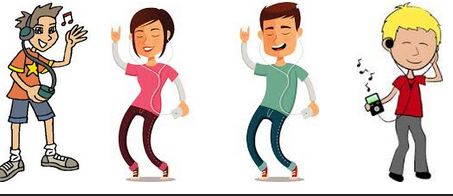
\includegraphics[scale = 0.5]{pic}	
  \centering
\end{figure}	
	
\end{frame}

\section{Related Works}

\begin{frame}{Related Works}
  
  \begin{itemize}
  \item {
    There is some existing work dealing with audio mood classification.
  } \pause
  \item {
    Also some recent literature about mood detection in text
  } 
  
  
  
  \end{itemize}
\end{frame}


\begin{frame}{Related Works}
  
  \begin{itemize}
  \item {
    Neumayer and Rauber have shown the complementarity of audio and lyrics in the context of genre classification
  } \pause
  \item {
    Logan et al. have investigated the properties of lyrics using Latent Semantic Analysis.
  } \pause
  
  \item {
    Natural genre clusters were discovered .Their conclusion was also that lyrics are useful for artist similarity searches.
    
  } \pause
  \item {
    Studies in cognitive neuropsychology also demonstrated the independence of both sources of information and so the potential complementarity of both melody and lyrics in the case of emotional expression.
  }
  
  \end{itemize}
\end{frame}

\begin{frame}{Related Works}
  
  \begin{itemize}
  \item {
    But very little has been done so far to address the automatic classification of lyrics according to their mood. 
  }
  
  \item {
    We have found no prior articles studying the combination of lyrics and acoustic information for this particular classification purpose.
  } 
  
  
  \end{itemize}
\end{frame}



\section{Database}

\begin{frame}{Database}
According to the moods the songs are classified into four catagories.


	\begin{itemize}
	  \item {
		Happy
	  } 
	  \item<2-> {
		Relaxed
	  } 
	  \item<3-> {
		Sad
	  } 
	  \item<4-> {
		Angry
	  }
	  
	\end{itemize}

	
	\begin{columns}
	\column{0.25\textwidth}
	
\includegraphics{happy}
	\pause
	


	\column{0.25\textwidth}
	
\includegraphics{relaxed}
	\pause


	\column{0.25\textwidth}
	
\includegraphics{sad}
	\pause


	\column{0.25\textwidth}
	
\includegraphics{angry}
	\pause
  	\end{columns}
\end{frame}

\begin{frame}{Database}

For choosing songs , the folloowing criterias are maintained in order to get a more accurate result

	\begin{itemize}
	\item
	{
		Songs were collected from last.fm with their maintained tags
	} \pause
	\item
	{
		Only songs having English lyrics and an entry in LyricWiki were selected 
	} \pause
	\item
	{
		The tags of the songs were once more evaluated by listeners to ensure more accuracy
	} \pause
	\item
	{
		In total, 17 different evaluators participated and an average of 71.3\% of the songs originally selected from last.fm were validated
	} \pause
	\item
	{
		The database is composed of 1000 songs divided between 4 categories. An equal distribution of these binary classes was used.
	}
	\end{itemize}

\end{frame}

\section{Classification}

\subsection{Audio Classification}

\begin{frame}{Audio Classification}
  \begin{itemize}
  \item {
    To classify music by mood a state-of-the-art audio classification algorithm was used in a supervised learning approach.
  }
  \item 
  {
  	The features and the classifier were selected according to current litterature
    
  }
  \item 
  {
  	The results from the Audio Mood Classification evaluation task held by the Music Information Retrieval Evaluation eXchange (MIREX)
    
  }
  \end{itemize}
\end{frame}

\begin{frame}{Audio Classification}
  \begin{itemize}
  \item 
  {
    In order to classify the music from acoustical information, we first extracted audio features of different kinds:
    \begin{itemize}
    \item
    {
    	Timbral (for instance MFCC, spectral centroid)
    }
    \item
   	{
   		Rhythmic(for example tempo, onset rate)
   	}
    \item
    {
    	Tonal (like Harmonic Pitch Class Profiles)
    }
    \item
   	{
   		Temporal descriptors
   	}
    \end{itemize}
  }

  
  
  \end{itemize}
\end{frame}


\begin{frame}{Audio Classification}
	\begin{itemize}
	\item 
	  {
	  	Classifiers were used like Support Vector Machines(SVM) , Random Forest or Logistic Regres
	  	\begin{figure}
	  	\centering
	  	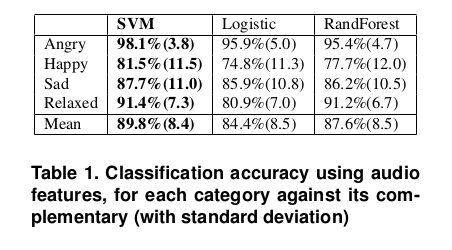
\includegraphics[scale = 0.5 ]{table1}
	  	\end{figure}
	  	Among them SVM gives us the best result.
	  	
	  }
 	\end{itemize}
\end{frame}

\subsection{Lyric Classification}

% You can reveal the parts of a slide one at a time
% with the \pause command:
\subsubsection{Experiment 1}

\begin{frame}{Experiment 1}{Classification based on similarity using Lucene}
  \begin{itemize}
  \item {
    The representation of the songs is reduced to a bag of words i.e. the set of words or terms used in a song as well as their frequency
  }
  \item 
  {
  	This is then used, with the help of the Lucene document retrieval system [4] , to rank documents by their similarity   
    
  }
  \item
  {
  	More importance was attributed to those terms that are frequent in the given song, but less frequent overall in the collection
  }
  
  
  \end{itemize}
\end{frame}

\begin{frame}{Experiment 1}{Result}
We conducted experiments with varying numbers of similar documents (k) to be taken into account.
  \begin{itemize}
  \item {
    A low k provides less stability, as the predicted label depends strongly on individual examples from the collection
  }
  \item 
  {
  	Large ks on the other hand can mean that examples are taken into account that are not actually very similar (and thus representative) of the one that is to be classified
    
  }
  \end{itemize}
  The optimum depends on the application and the distribution of the datapoints and can not be easily predicted a-priori
  
\end{frame}


\begin{frame}{Experiment 1}{Result}
{\small As we are seeing , the prediction power of the similarity-based approach for lyrics remains limited, with averaged accuracy around 60\%. The most predictable catagory is "angry" and the least predictable is "sad".  }
	\begin{table}[tbh]
		\centering
		
		\begin{tabular}{|c|c|c|c|c|c|}
		\hline
		        & k=3(\%) & k=5(\%) & k=7(\%) & k=9(\%) & k=11(\%) \\ \hline
		  Angry & 69.5 & 67.5 & 69.0 & 68.5 & 67.0 \\ %\hline
		  Happy & 55.9 & 57.4 & 60.9 & 64.5 & 64.1\\ %\hline
		  Sad & 55.0 & 52.8 & 58.9 & 54.5 & 55.0\\ %\hline
		  Relaxed & 61.8 & 65.8 & 61.0 & 59.8 & 59.1 \\ \hline
		  Mean & 60.5 & 60.9 & 62.5 & 61.8 & 61.3 \\ \hline
		  
		  
		   
		
		
		\end{tabular}
		\caption{Classification accuracies using K - NN with a if.idf based distance on lyrics for different values of k}
	\end{table}  
\end{frame}

\begin{frame}{Experiment 1}{Limitations}
But there are some limitations :
\begin{itemize}
\item
{
	It is difficult to directly integrate the results
}
\item
{
	While the audio side, the featured vectors can be used with different clasification algorithms , this is not as easy case for the lyrics
}
\item
{
	Vocabulary size already reached 7000 words while more complete collections reach vocabulary sizes of several hundred thousand distinct words
}

\end{itemize}
\end{frame}



\subsubsection{Experiment 2}

\begin{frame}{Experiment 2}{Classification using Latent Semantic Analysis (LSA) }
One approach to deal with the dimensionality problem is to
  \begin{itemize}
  \item {
    project the lyrics into a lower-dimensional space that is manageable by generic classifiers
  }
  \item 
  {
  	project the data into a space of a given dimensionality using Latent Semantic Analysis (LSA)
    
  }
  \item
  {
  	maintain a good approximation of the distances between data points.

}
Experiments were conducted to determine the impact of the number of dimensions used in the LCA . As could be expected, performance (using lyrics alone) is very low for extremely low dimensionality and tends to improve with a greater number of dimensions.
  
  
  \end{itemize}
\end{frame}




\begin{frame}{Experiment 2}{Result}
{\small The use of LSA does not dramatically improve performance compared to our first experiment, depending on the category it can even be worse. The reduction in dimensionality does, however, provide more flexibility, as different types of classifiers can be used on the resulting representation. The results shown here use a reduction to 30 dimensions.}
	\begin{table}[tbh]
		\centering
		
		\begin{tabular}{|c|c|c|c|}
		\hline
		        & SVM(\%) & Logistic(\%) & RandForest(\%) \\ \hline
		  Angry & 62.1(9.1) & 62.0(10.2) & 61.3(11.5) \\ %\hline
		  Happy & 55.2(10.3) & 54.1(12.5) & 54.8(10.7) \\ %\hline
		  Sad & 66.4(9.7) & 65.3(11.0) & 56.7(12.1) \\ %\hline
		  Relaxed & 57.5(8.2) & 57.3(9.1) & 56.8(9.79) \\ \hline
		  Mean & 61.3(9.3) & 59.7(10.7) & 57.4(11.0) \\ \hline
		  
		  
		   
		
		
		\end{tabular}
		\caption{Classification accuracies using LSA}
	\end{table}  
\end{frame}


\begin{frame}{Experiment 2}{Limitations}
But there are some limitations :
\begin{itemize}
\item
{
	If our mood categories do not relate to clusters of songs that would be considered similar according to the metrics used in document retrieval
} \pause
\item
{
	This severally limits the potential of any approaches that are based on document distances with tf.idf weighting
} \pause
\item
{
	LSA doesn't overcome this problem as the distances between the data points in the projected space directly reflect their tf.idf based distance used as a basic for the transformation
}

\end{itemize}
\end{frame}


\subsubsection{Experiment 3}
\begin{frame}{Experiment 3}{Classification using Language Model Differences(LMD)}

 
  \begin{itemize}
  
  \item 
  {
  	 Distances between songs based on lyrics cannot separate our mood categories very well
  }
  \item
  {
  	But lyrics convey other types of information to be exploited in persuing their separation according to mood.
  }
  \item {
     In order to assess their potential the language models corresponding to the different categories were analyzed 
  }
  
  
  \end{itemize}
\end{frame}


\begin{frame}{Experiment 3}{Classification using Language Model Differences(LMD)}
{\small Figure 1 shows document frequencies for the 200 most frequent terms in the angry category compared to the frequencies to the not angry category}
\begin{figure}
\centering
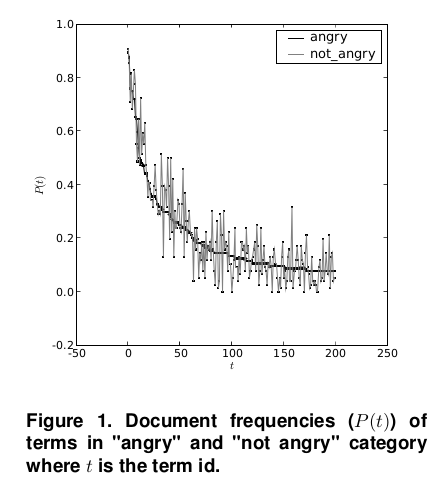
\includegraphics[scale = 0.28]{graph1}
\end{figure} 

\end{frame}

\begin{frame}{Experiment 3}{Classification using Language Model Differences(LMD)}
  \begin{itemize}
  \item {
    When  comparing two language models, the simplest approach is to calculate the difference in document frequency for all terms.  
  }
  \item 
  {
  	This can be computed either as an abosolute difference in document frequency for all terms.
Example of terms ranked by absloute difference:


	\begin{itemize}
	\item
	{
		\textit{angry:} world,die,death,control,...
	}
	\item
	{
		\textit{not angry:} me,love,i'm,can,could,so,but,...
	}
	\end{itemize}
	Examples of terms ranked by relative difference:
	\begin{itemize}
	\item
	{
		\textit{angry:} realms,bear,four,...
	}
	\item
	{
		\textit{not angry:} chillin,nursery,hanging,...
	}
	\end{itemize}
  }
  
  
  \end{itemize}
\end{frame}

\begin{frame}{Experiment 3}{Classification using Language Model Differences(LMD)}

Here are some necessary equaions to evaluate the absolute difference and relative
\begin{figure}
\centering
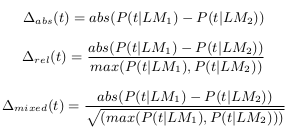
\includegraphics{eq}
\end{figure}

\end{frame}


\begin{frame}{Experiment 3}{Result}

{\tiny For each category, we selected the n terms with the highest ∆ mixed . We obtained a vector representation with n dimensions that can be used with different classifiers. We made 10 runs of 10-fold cross-validation (this includes the term selection, of course) and tried different values n.}
	\begin{table}[tbh]
		\centering
		
		\begin{tabular}{|c|c|c|c|}
		\hline
		        & SVM(\%) & Logistic(\%) & RandForest(\%) \\ \hline
		  Angry & 77.9(10.3) & 60.6(12.0) & 71.0(11.5) \\ %\hline
		  Happy & 80.8(12.1) & 67.5(13.3) & 70.8(11.4) \\ %\hline
		  Sad & 84.4(11.2) & 83.9(7.0) & 75.1(12.9) \\ %\hline
		  Relaxed & 79.7(9.5) & 71.3(10.5) & 78.0(9.5) \\ \hline
		  Mean & 80.7(10.8) & 70.8(10.7) & 73.7(11.3) \\ \hline
		\end{tabular}
		\caption{Classification performances using the 100 most discriminant terms}
	\end{table} 
\end{frame}



\section{Combining Audio and Lyric Information}

\begin{frame}{Combining Audio and Lyric Information}

We used two approaches to integrate these two information sources.

\begin{itemize}
\item
{
	The first one used separate predictions for
audio and lyrics and combined them through voting.
	
}
\item
{
	The second approach was to combine all features in the same space, having a vector composed of both audio and lyrics features. This allowed to use audio and lyrics information within one classifier
	
}

Only the second one is reported here.
\end{itemize}

\end{frame}

\subsection{Mixed Feature Space}

\begin{frame}{Combining Audio and Lyric Information}
Having audio and lyrics information in the same vector allows to exploit interdependencies between aspects from both modalities

\begin{itemize}
\item
{
	the combination of the language
model differences with the audio descriptors yielded to rel-
atively good results.
	
}
\item
{
	This combination gives significant improvements over both individual approaches, leveraging the complementary information available from audio and lyrics, at least for two of the four categories: “happy” and “sad” with both a sig- nificant (p less than 0.05 using a Paired T-Test) overall increase around 5\% for both
	
}
\item
{
	For the angry and relaxed categories
there is also a slight increase in classification performance
	
	
}
\end{itemize}
\end{frame}
\begin{frame}{Combining Audio and Lyric Information}
\begin{itemize}
\item
{
	However, the extremely high baseline of over 98\% accuracy on audio alone for the “angry” category, as well as the large difference in performance between lyrics and audio for “relax” limits the benefits of using a hybrid method

}

Only the second one is reported here.
\end{itemize}

\end{frame}


\begin{frame}{Experiment 3}{Result}

{\tiny For each category we show the accuracy of the SVM classifier for the audio analysis, for the lyrics analysis, and for the multimodal approach combining both. As in the previous experiments, the accuracies shown Table \ref{table:last} are averages over the 10 runs of 10-fold cross-validation.}
	\begin{table}[tbh]
		\centering
		\label{table:last}
		
		\begin{tabular}{|c|c|c|c|}
		\hline
		        & Audio(\%) & Lyrics(\%) & Mixed(\%) \\ \hline
		  Angry & 98.1(3.8) & 77.9(10.3 & 98.39(3.7)) \\ \hline
		  Happy & 81.5(11.5) & 80.8(11.2) & 86.8(10.6) \\ \hline
		  Sad &  87.7(11.0) & 84.4(11.2) & 92.8(8.7)\\ \hline
		  Relaxed & 91.4(7.30) & 79.7(9.5) & 91.7(7.1) \\ \hline

		\end{tabular}
		\caption{Classification accuracies using audio features, lyrics with language model differences and finally a mixed feature space both.}
	\end{table} 
\end{frame}


% Placing a * after \section means it will not show in the
% outline or table of contents.
\section{Summary}

\begin{frame}{Summary}
  \begin{itemize}
  \item
  {
  	This multimodal approach increases the performances for all the mood categories. 
  }  
  \item
    There are more work to be done with lyric modal approach to classify the mood of the songs. 
  
  \end{itemize}
  
  
\end{frame}



% All of the following is optional and typically not needed. 



\end{document}




